\chapter{وارد کردن فهرست اختصارات}
در این استایل برای تولید فهرست اختصارات از بسته {\lr{glossaries}} استفاده کنید. مراحل تولید فهرست اختصارات بسیار ساده و راحت است. این مراحل به شرح زیر می باشد. 
\begin{itemize}
\arcm
در فایل  ‎\lr{abbr}‎ که در پوشه ‎\lr{Chapters}‎ قرار دارد اختصارات مورد نظر خود را تعریف کنید. برای مثال:
\begin{latin}
\verb+ \newacronym{PSNR}{PSNR}{Peak Signal to Noise Ratio}+
\end{latin}

عنصر اول تعریف فوق، برچسب اختصار، مورد دومی خود اختصار و سومی باز شده آن است. 
\arcm
در هر جای متن که تمایل دارید با دستور  ‎\lr{gls}‎‌و برچسب کلمه اختصار مورد نظر آن را وارد کنید. مثلا:
\verb+\gls{PSNR}+
در این صورت هر جا که این دستور را بنویسید، کلمه ‎\lr{PSNR}‎‌ قرار داده می‌شود. در اولین مکانی که این کلمه را بکار برده‌اید، پاورقی می خورد و به صورت اتوماتیک این کلمه به فهرست اختصارات اضافه می‌شود.
\arcm
در انتهای نیز دنباله زیر را برای تولید فهرست اختصارات انجام دهید:
\begin{LTR}
\begin{itemize}
\tree
\verb+ xelatex -interaction=nonstopmode -synctex=-1 %.tex+
\tree
\verb+ xindy -M %.xdy -t %.nlg -o %.not %.ntn +
\tree
\verb+ xelatex -interaction=nonstopmode -synctex=-1 %.tex+
\tree
\verb+ xelatex -interaction=nonstopmode -synctex=-1 %.tex+
\end{itemize}
\end{LTR}
\end{itemize}
دستور 
\begin{LTR}
\verb+ xelatex -interaction=nonstopmode -synctex=-1 %.tex+
\end{LTR}

همانی است که با   ‎\lr{QuickBuild}‎ زدن اجرا می‌شود. دستور دومی را باید اضافه کنید. برای این کار مثلا برای مثال برای ‎\lr{TexStudio}‎، به منوی ‎\lr{option}‎ و سپس منوی ‎\lr{Configure Texstudio}‎ بروید. در قسمت ‎\lr{Build}‎ و در بخش ‎\lr{User Command}‎ این دستور را اضافه کنید. شکل زیر را مشاهده کنید. 
\begin{figure}[H]
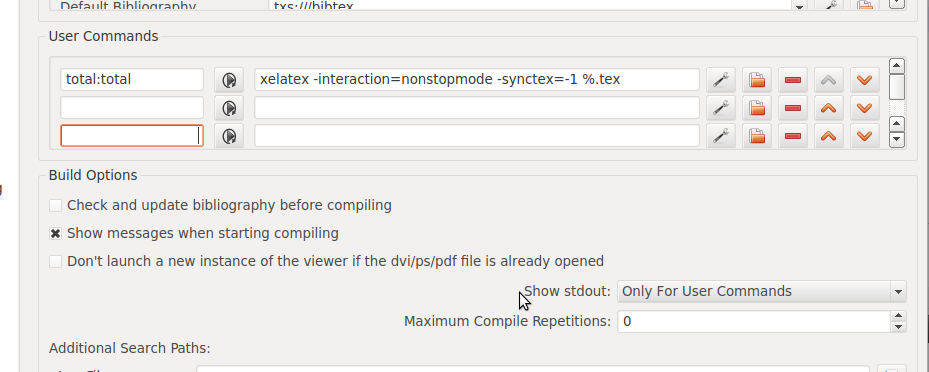
\includegraphics[width=0.9\linewidth]{../Pic/a}
\end{figure}

